\documentclass[journal,12pt,twocolumn]{IEEEtran}

\usepackage{setspace}
\usepackage{gensymb}
\singlespacing
\usepackage[cmex10]{amsmath}

\usepackage{amsthm}

\usepackage{mathrsfs}
\usepackage{txfonts}
\usepackage{stfloats}
\usepackage{bm}
\usepackage{cite}
\usepackage{cases}
\usepackage{subfig}
\usepackage{paralist}
\usepackage{longtable}
\usepackage{multirow}

\usepackage{enumitem}
\usepackage{mathtools}
\usepackage{steinmetz}
\usepackage{tikz}
\usepackage{circuitikz}
\usepackage{verbatim}
\usepackage{tfrupee}
\usepackage[breaklinks=true]{hyperref}
\usepackage{graphicx}
\usepackage{tkz-euclide}

\usetikzlibrary{calc,math}
\usepackage{listings}
    \usepackage{color}                                            %%
    \usepackage{array}                                            %%
    \usepackage{longtable}                                        %%
    \usepackage{calc}                                             %%
    \usepackage{multirow}                                         %%
    \usepackage{hhline}                                           %%
    \usepackage{ifthen}                                           %%
    \usepackage{lscape}     
\usepackage{multicol}
\usepackage{chngcntr}


\usetikzlibrary{calc,math}
\usepackage{listings}
    \usepackage{color}                                            %%
    \usepackage{array}                                            %%
    \usepackage{longtable}                                        %%
    \usepackage{calc}                                             %%
    \usepackage{multirow}                                         %%
    \usepackage{hhline}                                           %%
    \usepackage{ifthen}                                           %%
    \usepackage{lscape}     
\usepackage{multicol}
\usepackage{chngcntr}

\DeclareMathOperator*{\Res}{Res}

\renewcommand\thesection{\arabic{section}}
\renewcommand\thesubsection{\thesection.\arabic{subsection}}
\renewcommand\thesubsubsection{\thesubsection.\arabic{subsubsection}}

\renewcommand\thesectiondis{\arabic{section}}
\renewcommand\thesubsectiondis{\thesectiondis.\arabic{subsection}}
\renewcommand\thesubsubsectiondis{\thesubsectiondis.\arabic{subsubsection}}


\hyphenation{op-tical net-works semi-conduc-tor}
\def\inputGnumericTable{}                                 %%

\lstset{
%language=C,
frame=single, 
breaklines=true,
columns=fullflexible
}
\begin{document}

\newcommand{\BEQA}{\begin{eqnarray}}
\newcommand{\EEQA}{\end{eqnarray}}
\newcommand{\define}{\stackrel{\triangle}{=}}
\bibliographystyle{IEEEtran}
\raggedbottom
\setlength{\parindent}{0pt}
\providecommand{\mbf}{\mathbf}
\providecommand{\pr}[1]{\ensuremath{\Pr\left(#1\right)}}
\providecommand{\qfunc}[1]{\ensuremath{Q\left(#1\right)}}
\providecommand{\sbrak}[1]{\ensuremath{{}\left[#1\right]}}
\providecommand{\lsbrak}[1]{\ensuremath{{}\left[#1\right.}}
\providecommand{\rsbrak}[1]{\ensuremath{{}\left.#1\right]}}
\providecommand{\brak}[1]{\ensuremath{\left(#1\right)}}
\providecommand{\lbrak}[1]{\ensuremath{\left(#1\right.}}
\providecommand{\rbrak}[1]{\ensuremath{\left.#1\right)}}
\providecommand{\cbrak}[1]{\ensuremath{\left\{#1\right\}}}
\providecommand{\lcbrak}[1]{\ensuremath{\left\{#1\right.}}
\providecommand{\rcbrak}[1]{\ensuremath{\left.#1\right\}}}
\theoremstyle{remark}
\newtheorem{rem}{Remark}
\newcommand{\sgn}{\mathop{\mathrm{sgn}}}
\providecommand{\abs}[1]{\vert#1\vert}
\providecommand{\res}[1]{\Res\displaylimits_{#1}} 
\providecommand{\norm}[1]{\lVert#1\rVert}
%\providecommand{\norm}[1]{\lVert#1\rVert}
\providecommand{\mtx}[1]{\mathbf{#1}}
\providecommand{\mean}[1]{E[ #1 ]}
\providecommand{\fourier}{\overset{\mathcal{F}}{ \rightleftharpoons}}
%\providecommand{\hilbert}{\overset{\mathcal{H}}{ \rightleftharpoons}}
\providecommand{\system}{\overset{\mathcal{H}}{ \longleftrightarrow}}
	%\newcommand{\solution}[2]{\textbf{Solution:}{#1}}
\newcommand{\solution}{\noindent \textbf{Solution: }}
\newcommand{\cosec}{\,\text{cosec}\,}
\providecommand{\dec}[2]{\ensuremath{\overset{#1}{\underset{#2}{\gtrless}}}}
\newcommand{\myvec}[1]{\ensuremath{\begin{pmatrix}#1\end{pmatrix}}}
\newcommand{\mydet}[1]{\ensuremath{\begin{vmatrix}#1\end{vmatrix}}}
\numberwithin{equation}{subsection}
\makeatletter
\@addtoreset{figure}{problem}
\makeatother
\let\StandardTheFigure\thefigure
\let\vec\mathbf
\renewcommand{\thefigure}{\theproblem}
\def\putbox#1#2#3{\makebox[0in][l]{\makebox[#1][l]{}\raisebox{\baselineskip}[0in][0in]{\raisebox{#2}[0in][0in]{#3}}}}
     \def\rightbox#1{\makebox[0in][r]{#1}}
     \def\centbox#1{\makebox[0in]{#1}}
     \def\topbox#1{\raisebox{-\baselineskip}[0in][0in]{#1}}
     \def\midbox#1{\raisebox{-0.5\baselineskip}[0in][0in]{#1}}
\vspace{3cm}
\title{AI1103-Assignment 3}
\author{Name: Avula Mohana Durga Dinesh Reddy , Roll Number: CS20BTECH11005}
\maketitle
\newpage
\bigskip
\renewcommand{\thefigure}{\theenumi}
\renewcommand{\thetable}{\theenumi}
Download all python codes from 
\begin{lstlisting}
https://github.com/DineshAvulaMohanaDurga/AI1103/blob/main/assignment_3/codes/ai1103_assignment3.py
\end{lstlisting}
%
and latex codes from 
%
\begin{lstlisting}
https://github.com/DineshAvulaMohanaDurga/AI1103/blob/main/assignment_3/main.tex
\end{lstlisting}
\section{Question}
\brak{GATE-2021\brak{ME, set-1} problem-5} Consider a binomial random variable X. If \textbf{$X_1,X_2,...,X_n$} are independent and identically distributed samples from the distribution of \textbf{X} with sum Y=$\Sigma_{i=1}^n X_i$, then the distribution of \textbf{Y} as $n\rightarrow \infty$ can be approximated as
\begin{enumerate}
    \item Exponential
    \item Bernoulli 
    \item Binomial
    \item Normal
\end{enumerate}

\section{Answer}
Given a binomial random variable \textbf{X} 
\begin{align}
\Rightarrow X \sim B\brak{r,p}
\end{align}

also given that $X_1,X_2,...,X_n$ are independent and identically distributed samples 
\begin{align}
    \Rightarrow X_1=X_2=...=X_n=X \sim B\brak{r,p}
\end{align}
also given that
\begin{align}
Y&=\displaystyle\sum_{i=1}^n X_i
\end{align}
We know that the characteristic equation of binomial trials with n elements is \begin{align}
    \phi_X\brak{t}&={\brak{1-p+p e^{it}}}^n
\end{align}
consider two sets of Bernoulli trials containing $r_1 \& r_2$ elements respectively where both trials have the same probability 'p'$\brak{X\sim B\brak{r_1,p},Y\sim\brak{r_2,p}}$. Now considering both as a whole set
\begin{align}
B\brak{r_1,p}+B\brak{r_2,p}&=\Phi_{X+Y}\brak{t}\\
&=\Phi_X\brak{t}\times \Phi_Y\brak{t}\nonumber\\
&={\brak{1-p+p e^{it}}}^{r_1}\nonumber\\
&\hspace*{1cm}\times {\brak{1-p+p e^{it}}}^{r_2}\\
&={\brak{1-p+p e^{it}}}^{r_1+r_2}\\
&=B\brak{r_1+r_2,p}\nonumber\\
\therefore B\brak{r_1,p}+B\brak{r_2,p}&=B\brak{r_1+r_2,p}
\end{align}
using this recursively we get
\begin{align}
    Y&=B\brak{r n,p}
\end{align}
$\Rightarrow$ using standard formulae
\begin{align}
\text{mean of Y } \mu_Y&=nrp \nonumber\\
\text{and variance } \sigma^2_Y&=nrp\brak{1-p}
\end{align}
By central limit theorem\brak{CLT}
\begin{align}
    Z_n &= \sqrt{n}\brak{\frac{\frac{Y}{n} - \mu_Y}{\sigma_Y}}\nonumber\\
    &=\frac{Y-n \mu_Y}{\sqrt{n} \sigma_Y}
\end{align}
$\lim_{n \rightarrow \infty} Z_n \sim N\brak{0,1}$ \\
Which is a normal distribution\\
$\therefore$ the correct answer is option D
\begin{figure}[ht]
    \centering
    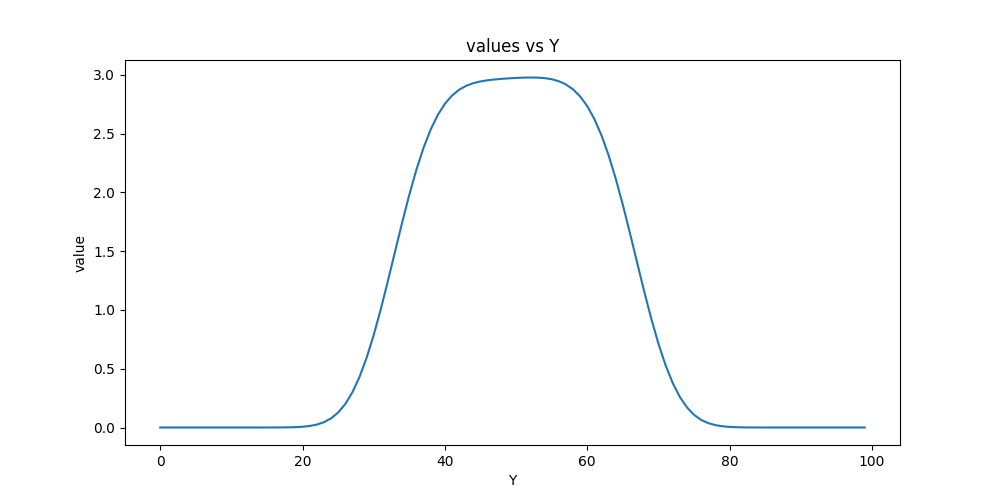
\includegraphics[width=0.5\textwidth]{figure1.png}
    \caption{distribution of Y}
    \label{fig:my_label}
\end{figure}
\end{document}